\documentclass[10pt]{beamer}\usepackage[]{graphicx}\usepackage[]{color}
%% maxwidth is the original width if it is less than linewidth
%% otherwise use linewidth (to make sure the graphics do not exceed the margin)
\makeatletter
\def\maxwidth{ %
  \ifdim\Gin@nat@width>\linewidth
    \linewidth
  \else
    \Gin@nat@width
  \fi
}
\makeatother

\definecolor{fgcolor}{rgb}{0.345, 0.345, 0.345}
\newcommand{\hlnum}[1]{\textcolor[rgb]{0.686,0.059,0.569}{#1}}%
\newcommand{\hlstr}[1]{\textcolor[rgb]{0.192,0.494,0.8}{#1}}%
\newcommand{\hlcom}[1]{\textcolor[rgb]{0.678,0.584,0.686}{\textit{#1}}}%
\newcommand{\hlopt}[1]{\textcolor[rgb]{0,0,0}{#1}}%
\newcommand{\hlstd}[1]{\textcolor[rgb]{0.345,0.345,0.345}{#1}}%
\newcommand{\hlkwa}[1]{\textcolor[rgb]{0.161,0.373,0.58}{\textbf{#1}}}%
\newcommand{\hlkwb}[1]{\textcolor[rgb]{0.69,0.353,0.396}{#1}}%
\newcommand{\hlkwc}[1]{\textcolor[rgb]{0.333,0.667,0.333}{#1}}%
\newcommand{\hlkwd}[1]{\textcolor[rgb]{0.737,0.353,0.396}{\textbf{#1}}}%
\let\hlipl\hlkwb

\usepackage{framed}
\makeatletter
\newenvironment{kframe}{%
 \def\at@end@of@kframe{}%
 \ifinner\ifhmode%
  \def\at@end@of@kframe{\end{minipage}}%
  \begin{minipage}{\columnwidth}%
 \fi\fi%
 \def\FrameCommand##1{\hskip\@totalleftmargin \hskip-\fboxsep
 \colorbox{shadecolor}{##1}\hskip-\fboxsep
     % There is no \\@totalrightmargin, so:
     \hskip-\linewidth \hskip-\@totalleftmargin \hskip\columnwidth}%
 \MakeFramed {\advance\hsize-\width
   \@totalleftmargin\z@ \linewidth\hsize
   \@setminipage}}%
 {\par\unskip\endMakeFramed%
 \at@end@of@kframe}
\makeatother

\definecolor{shadecolor}{rgb}{.97, .97, .97}
\definecolor{messagecolor}{rgb}{0, 0, 0}
\definecolor{warningcolor}{rgb}{1, 0, 1}
\definecolor{errorcolor}{rgb}{1, 0, 0}
\newenvironment{knitrout}{}{} % an empty environment to be redefined in TeX

\usepackage{alltt}

\usetheme{metropolis}

% Comment out for slides
% \usepackage{pgfpages} 	
% \pgfpagesuselayout{4 on 1} 	

\usepackage{booktabs}
\usepackage[scale=2]{ccicons}

\usepackage{pgfplots}
\usepgfplotslibrary{dateplot}

\usepackage{xspace}
\newcommand{\themename}{\textbf{\textsc{metropolis}}\xspace}

\usepackage{color}
\definecolor{LUBlue}{RGB}{0,74,136}
%
\usecolortheme[named=LUBlue]{structure} 
%
%\setbeamercolor*{palette primary}{fg=white, bg=LUBlue}%gray!15!white}
%
%\setbeamercolor{titlelike}{parent=palette primary}
\setbeamercolor{frametitle}{bg=LUBlue}
%\setbeamercolor{frametitle right}{bg=gray!60!white}

\graphicspath{{./figures/}}
\usepackage{booktabs}% http://ctan.org/pkg/booktabs
\usepackage{array}% http://ctan.org/pkg/array
\newcolumntype{M}{>{\centering\arraybackslash}m{\dimexpr.05\linewidth-2\tabcolsep}}

\title{Exploratory Data Analysis}
\subtitle{Part 1: Tidy data + Univariate graphics}
\date{}
\author{Math 445, Spring 2017}
\titlegraphic{\hfill
\includegraphics[height=1.5cm]{LULogo}}

\usepackage[makeroom]{cancel}
\IfFileExists{upquote.sty}{\usepackage{upquote}}{}
\begin{document}






\maketitle

%\begin{frame}{Overview}
%  \setbeamertemplate{section in toc}[sections numbered]
%  \tableofcontents[hideallsubsections]
%\end{frame}

% ---------------------------------------------------
% ---------------------------------------------------
\section{Loading Data into R}

% --------------------------------------------------- Slide --

\begin{frame}[fragile]{Flight Delays}

Overview: All departures from LaGuardia during May and June 2009

\bigskip

\begin{tabular}{l l} \hline
Variable name & Description\\ \hline
Carrier     & UA = United Airlines, AA = American Airlines\\
FlightNo    & Flight number\\
Destination & Destination airport code\\
DepartTime  & Schedule departure time (4 hr intervals)\\
Day         & Day of the week\\
Month       & May or June\\
FlightLength & Duration of flight (min.)\\
Delay       & Minutes flight delayed (neg. for early dept.)\\
Delayed30   & Was the flight delayed at least 30 min?\\
\hline
\end{tabular}
\end{frame}

% --------------------------------------------------- Slide --

\begin{frame}[fragile]{read.table}

\begin{itemize}
\item  If you already have a data set saved, then you can simply load
the data set into R.
\item[]
\item  Example: If you wanted to read in the \texttt{FlightDelays.csv} data set, then run the command (substituting the approriate file path)

\begin{knitrout}\scriptsize
\definecolor{shadecolor}{rgb}{0.969, 0.969, 0.969}\color{fgcolor}\begin{kframe}
\begin{alltt}
\hlstd{flights} \hlkwb{<-} \hlkwd{read.table}\hlstd{(}\hlkwc{file} \hlstd{=} \hlstr{"../../data/FlightDelays.csv"}\hlstd{,} \hlkwc{sep} \hlstd{=} \hlstr{","}\hlstd{,} \hlkwc{header} \hlstd{=} \hlnum{TRUE}\hlstd{)}
\end{alltt}
\end{kframe}
\end{knitrout}
\item[]
\item You can use \texttt{file.choose()} to get a pop-up window for file selection

\begin{knitrout}\scriptsize
\definecolor{shadecolor}{rgb}{0.969, 0.969, 0.969}\color{fgcolor}\begin{kframe}
\begin{alltt}
\hlstd{flights} \hlkwb{<-} \hlkwd{read.table}\hlstd{(}\hlkwc{file} \hlstd{=} \hlkwd{file.choose}\hlstd{(),} \hlkwc{sep} \hlstd{=} \hlstr{","}\hlstd{,} \hlkwc{header} \hlstd{=} \hlnum{TRUE}\hlstd{)}
\end{alltt}
\end{kframe}
\end{knitrout}

WARNING: This will not work in an R markdown file.

\end{itemize}

\end{frame}


% --------------------------------------------------- Slide --
\begin{frame}[fragile]{read.table}

\begin{itemize}
\item \texttt{read.table} is our workhorse function, and can read in numerous file types

\item[]

\item for different file types you will need to specify different field separator characters:\\

\item[]

\begin{tabular}{l  l} \hline
  Separator    & Description\\ \hline
  \texttt{sep = " "}  & white space separated\\
  \verb|sep = "\t"| & tab separated\\
  \texttt{sep = ","}  & comma separated files (.csv) \\ \hline
\end{tabular}

\item[]

\item Use \texttt{header = TRUE} if there are column names

\item[]

\item \texttt{read.csv} is a shortcut to \texttt{read.table} where \texttt{sep = ","} and \texttt{header = TRUE}
\end{itemize}

\end{frame}


% --------------------------------------------------- Slide --
\begin{frame}[fragile]{Did it work?}

The following commands provide useful ways to check that the data loaded correctly

\begin{knitrout}\small
\definecolor{shadecolor}{rgb}{0.969, 0.969, 0.969}\color{fgcolor}\begin{kframe}
\begin{alltt}
\hlkwd{dim}\hlstd{(flights)}
\hlkwd{nrow}\hlstd{(flights)}
\hlkwd{ncol}\hlstd{(flights)}
\hlkwd{str}\hlstd{(flights)}
\hlkwd{head}\hlstd{(flights)}
\end{alltt}
\end{kframe}
\end{knitrout}

\end{frame}

% --------------------------------------------------- Slide --
\begin{frame}[fragile]{Textbook data}

The \texttt{resampledata} R package contains the data sets discussed in the textbook.

\begin{knitrout}\small
\definecolor{shadecolor}{rgb}{0.969, 0.969, 0.969}\color{fgcolor}\begin{kframe}
\begin{alltt}
\hlcom{# Install (only do once)}
\hlkwd{install.packages}\hlstd{(}\hlstr{"resampledata"}\hlstd{)}

\hlcom{# Load}
\hlkwd{library}\hlstd{(resampledata)}
\end{alltt}
\end{kframe}
\end{knitrout}


\end{frame}

% ---------------------------------------------------
% ---------------------------------------------------
\section{Tidy Data}


% --------------------------------------------------- Slide --
\begin{frame}[fragile]{Data tables}

\begin{itemize}
\item A row is always a \alert{case}
\item A column is always a \alert{variable}
\end{itemize}




\begin{knitrout}\scriptsize
\definecolor{shadecolor}{rgb}{0.969, 0.969, 0.969}\color{fgcolor}\begin{kframe}
\begin{alltt}
\hlkwd{head}\hlstd{(flights)}
\end{alltt}
\begin{verbatim}
##   ID Carrier FlightNo Destination DepartTime Day Month FlightLength Delay Delayed30
## 1  1      UA      403         DEN      4-8am Fri   May          281    -1        No
## 2  2      UA      405         DEN     8-Noon Fri   May          277   102       Yes
## 3  3      UA      409         DEN      4-8pm Fri   May          279     4        No
## 4  4      UA      511         ORD     8-Noon Fri   May          158    -2        No
## 5  5      UA      667         ORD      4-8am Fri   May          143    -3        No
## 6  6      UA      669         ORD      4-8am Fri   May          150     0        No
\end{verbatim}
\end{kframe}
\end{knitrout}

\end{frame}

% --------------------------------------------------- Slide --
\begin{frame}[fragile]{Cases}

A case contains all values measured on the same unit across attributes (variables)

\begin{knitrout}\scriptsize
\definecolor{shadecolor}{rgb}{0.969, 0.969, 0.969}\color{fgcolor}\begin{kframe}
\begin{alltt}
\hlkwd{head}\hlstd{(flights)}
\end{alltt}
\begin{verbatim}
##   ID Carrier FlightNo Destination DepartTime Day Month FlightLength Delay Delayed30
## 1  1      UA      403         DEN      4-8am Fri   May          281    -1        No
## 2  2      UA      405         DEN     8-Noon Fri   May          277   102       Yes
## 3  3      UA      409         DEN      4-8pm Fri   May          279     4        No
## 4  4      UA      511         ORD     8-Noon Fri   May          158    -2        No
## 5  5      UA      667         ORD      4-8am Fri   May          143    -3        No
## 6  6      UA      669         ORD      4-8am Fri   May          150     0        No
\end{verbatim}
\end{kframe}
\end{knitrout}

\end{frame}

% --------------------------------------------------- Slide --
\begin{frame}[fragile]{Variables}

A variable contains all values that measure the same underlying attribute across cases

\begin{itemize}
\item categorical
\item quantitative
\end{itemize}

\begin{knitrout}\scriptsize
\definecolor{shadecolor}{rgb}{0.969, 0.969, 0.969}\color{fgcolor}\begin{kframe}
\begin{alltt}
\hlkwd{head}\hlstd{(flights)}
\end{alltt}
\begin{verbatim}
##   ID Carrier FlightNo Destination DepartTime Day Month FlightLength Delay Delayed30
## 1  1      UA      403         DEN      4-8am Fri   May          281    -1        No
## 2  2      UA      405         DEN     8-Noon Fri   May          277   102       Yes
## 3  3      UA      409         DEN      4-8pm Fri   May          279     4        No
## 4  4      UA      511         ORD     8-Noon Fri   May          158    -2        No
## 5  5      UA      667         ORD      4-8am Fri   May          143    -3        No
## 6  6      UA      669         ORD      4-8am Fri   May          150     0        No
\end{verbatim}
\end{kframe}
\end{knitrout}

\end{frame}

% --------------------------------------------------- Slide --
\begin{frame}[fragile]{Tidy data}

\begin{enumerate}
\item Each variable forms a column
\item Each case forms a row
\item Each type of case (observational unit) forms a table
\end{enumerate}

\begin{knitrout}\scriptsize
\definecolor{shadecolor}{rgb}{0.969, 0.969, 0.969}\color{fgcolor}\begin{kframe}
\begin{alltt}
\hlkwd{head}\hlstd{(flights)}
\end{alltt}
\begin{verbatim}
##   ID Carrier FlightNo Destination DepartTime Day Month FlightLength Delay Delayed30
## 1  1      UA      403         DEN      4-8am Fri   May          281    -1        No
## 2  2      UA      405         DEN     8-Noon Fri   May          277   102       Yes
## 3  3      UA      409         DEN      4-8pm Fri   May          279     4        No
## 4  4      UA      511         ORD     8-Noon Fri   May          158    -2        No
## 5  5      UA      667         ORD      4-8am Fri   May          143    -3        No
## 6  6      UA      669         ORD      4-8am Fri   May          150     0        No
\end{verbatim}
\end{kframe}
\end{knitrout}

\end{frame}

% ---------------------------------------------------
% ---------------------------------------------------
\section{Plotting data}

% --------------------------------------------------- Slide --
\begin{frame}[fragile]{ggplot2}

\begin{itemize}
\item I prefer using \texttt{ggplot2} graphics to the rather \texttt{base} graphics system used in the textbook.

\item If you are using your personal computer, you will need to install
this package before you use it the first time

\begin{knitrout}\small
\definecolor{shadecolor}{rgb}{0.969, 0.969, 0.969}\color{fgcolor}\begin{kframe}
\begin{alltt}
\hlkwd{install.packages}\hlstd{(}\hlstr{"ggplot2"}\hlstd{)}
\end{alltt}
\end{kframe}
\end{knitrout}

\item You will need to load this package at the beginning of each R session:

\begin{knitrout}\small
\definecolor{shadecolor}{rgb}{0.969, 0.969, 0.969}\color{fgcolor}\begin{kframe}
\begin{alltt}
\hlkwd{library}\hlstd{(ggplot2)}
\end{alltt}
\end{kframe}
\end{knitrout}

\end{itemize}

\end{frame}

% --------------------------------------------------- Slide --
\begin{frame}[fragile]{The layered grammar of graphics}

\begin{itemize}
\item \texttt{ggplot2} implements a layered grammar of graphics providing a unified approach to building plots in R

\item[]

\item There is a bit of a learning curve, but the logic behind it is very intuitive

$$\text{base layer} + \text{geometry} + \text{options}$$

\item[]
\item It's easiest to learn by example

\end{itemize}


\end{frame}


% --------------------------------------------------- Slide --
\begin{frame}[fragile]{Basic univariate graphics}

\begin{tabular}{ll} \hline
Variable type & Plot suggestions\\\hline
Categorical   & Bar chart\\
              & \\
Quantitative  & Histogram\\
              & Boxplot\\
              & Kernel density estimate\\ 
              & Quantile-quantile plots\\
              & Empirical CDF\\
\hline
\end{tabular}

\end{frame}

% --------------------------------------------------- Slide --
\begin{frame}[fragile]{Bar charts}

Basic bar chart

\begin{knitrout}\small
\definecolor{shadecolor}{rgb}{0.969, 0.969, 0.969}\color{fgcolor}\begin{kframe}
\begin{alltt}
\hlkwd{ggplot}\hlstd{(}\hlkwc{data} \hlstd{= flights,} \hlkwc{mapping} \hlstd{=} \hlkwd{aes}\hlstd{(}\hlkwc{x} \hlstd{= Carrier))} \hlopt{+}
  \hlkwd{geom_bar}\hlstd{()}
\end{alltt}
\end{kframe}
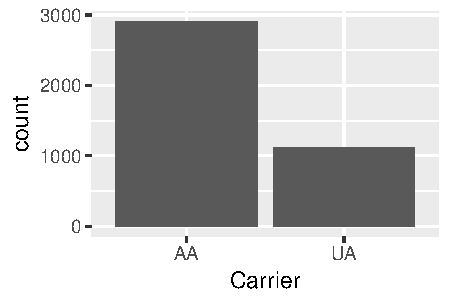
\includegraphics[width=\maxwidth]{figure/unnamed-chunk-14-1} 

\end{knitrout}

\end{frame}


% --------------------------------------------------- Slide --
\begin{frame}[fragile]{Bar charts}

You can also add options

\begin{knitrout}\small
\definecolor{shadecolor}{rgb}{0.969, 0.969, 0.969}\color{fgcolor}\begin{kframe}
\begin{alltt}
\hlkwd{ggplot}\hlstd{(}\hlkwc{data} \hlstd{= flights,} \hlkwc{mapping} \hlstd{=} \hlkwd{aes}\hlstd{(}\hlkwc{x} \hlstd{= Carrier,} \hlkwc{fill} \hlstd{= Carrier))} \hlopt{+}
  \hlkwd{geom_bar}\hlstd{()} \hlopt{+}
  \hlkwd{labs}\hlstd{(}\hlkwc{title} \hlstd{=} \hlstr{"Bar chart of flights by carrier"}\hlstd{)}
\end{alltt}
\end{kframe}
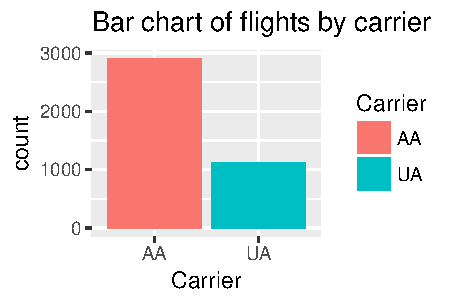
\includegraphics[width=\maxwidth]{figure/unnamed-chunk-15-1} 

\end{knitrout}

\end{frame}

% --------------------------------------------------- Slide --
\begin{frame}[fragile]{Histograms}


\begin{knitrout}\small
\definecolor{shadecolor}{rgb}{0.969, 0.969, 0.969}\color{fgcolor}\begin{kframe}
\begin{alltt}
\hlkwd{ggplot}\hlstd{(}\hlkwc{data} \hlstd{= flights,} \hlkwc{mapping} \hlstd{=} \hlkwd{aes}\hlstd{(}\hlkwc{x} \hlstd{= FlightLength))} \hlopt{+}
  \hlkwd{geom_histogram}\hlstd{()} \hlopt{+}
  \hlkwd{labs}\hlstd{(}\hlkwc{x} \hlstd{=} \hlstr{"Flight length (min)"}\hlstd{)}
\end{alltt}
\end{kframe}
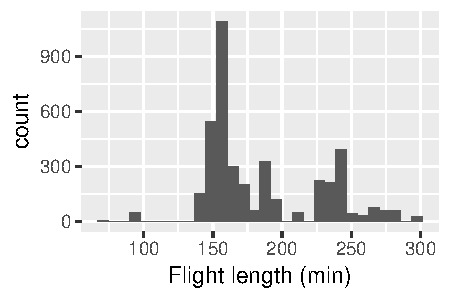
\includegraphics[width=\maxwidth]{figure/unnamed-chunk-16-1} 

\end{knitrout}

\end{frame}

\plain{Always experiment with the bin width}

% --------------------------------------------------- Slide --
\begin{frame}[fragile]{Histograms}

\begin{knitrout}\small
\definecolor{shadecolor}{rgb}{0.969, 0.969, 0.969}\color{fgcolor}\begin{kframe}
\begin{alltt}
\hlkwd{ggplot}\hlstd{(}\hlkwc{data} \hlstd{= flights,} \hlkwc{mapping} \hlstd{=} \hlkwd{aes}\hlstd{(}\hlkwc{x} \hlstd{= FlightLength),} \hlkwc{binwidth} \hlstd{=} \hlnum{30}\hlstd{)} \hlopt{+}
  \hlkwd{geom_histogram}\hlstd{()} \hlopt{+}
  \hlkwd{labs}\hlstd{(}\hlkwc{x} \hlstd{=} \hlstr{"Flight length (min)"}\hlstd{)}
\end{alltt}
\end{kframe}
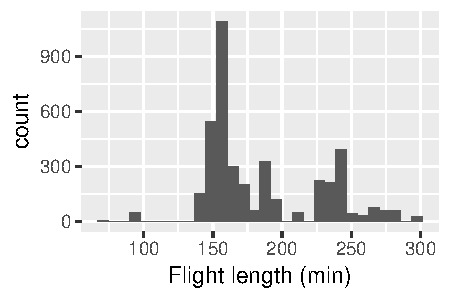
\includegraphics[width=\maxwidth]{figure/unnamed-chunk-17-1} 

\end{knitrout}

\end{frame}

% --------------------------------------------------- Slide --
\begin{frame}[fragile]{Kernel density estimates}

\begin{knitrout}\small
\definecolor{shadecolor}{rgb}{0.969, 0.969, 0.969}\color{fgcolor}\begin{kframe}
\begin{alltt}
\hlkwd{ggplot}\hlstd{(}\hlkwc{data} \hlstd{= flights,} \hlkwc{mapping} \hlstd{=} \hlkwd{aes}\hlstd{(}\hlkwc{x} \hlstd{= FlightLength))} \hlopt{+}
  \hlkwd{geom_density}\hlstd{()} \hlopt{+}
  \hlkwd{labs}\hlstd{(}\hlkwc{x} \hlstd{=} \hlstr{"Flight length (min)"}\hlstd{)}
\end{alltt}
\end{kframe}
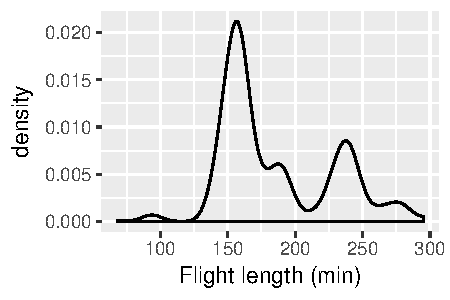
\includegraphics[width=\maxwidth]{figure/unnamed-chunk-18-1} 

\end{knitrout}

\end{frame}

% --------------------------------------------------- Slide --
\begin{frame}[fragile]{Histograms + Kernel densities}

\begin{knitrout}\scriptsize
\definecolor{shadecolor}{rgb}{0.969, 0.969, 0.969}\color{fgcolor}\begin{kframe}
\begin{alltt}
\hlkwd{ggplot}\hlstd{(}\hlkwc{data} \hlstd{= flights)} \hlopt{+}
  \hlkwd{geom_histogram}\hlstd{(}\hlkwc{mapping} \hlstd{=} \hlkwd{aes}\hlstd{(}\hlkwc{x} \hlstd{= FlightLength,} \hlkwc{y} \hlstd{= ..density..),} \hlkwc{binwidth} \hlstd{=} \hlnum{15}\hlstd{)} \hlopt{+}
  \hlkwd{geom_density}\hlstd{(}\hlkwc{mapping} \hlstd{=} \hlkwd{aes}\hlstd{(}\hlkwc{x} \hlstd{= FlightLength),} \hlkwc{colour} \hlstd{=} \hlstr{"orange"}\hlstd{)} \hlopt{+}
  \hlkwd{labs}\hlstd{(}\hlkwc{x} \hlstd{=} \hlstr{"Flight length (min)"}\hlstd{)}
\end{alltt}
\end{kframe}
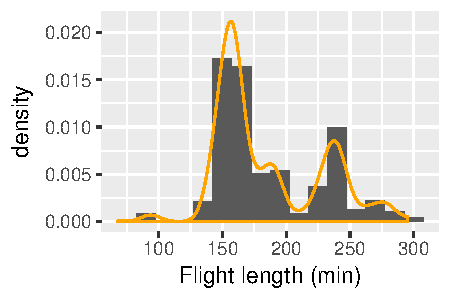
\includegraphics[width=\maxwidth]{figure/unnamed-chunk-19-1} 

\end{knitrout}

\end{frame}

% --------------------------------------------------- Slide --
\begin{frame}[fragile]{Boxplots}

\begin{knitrout}\scriptsize
\definecolor{shadecolor}{rgb}{0.969, 0.969, 0.969}\color{fgcolor}\begin{kframe}
\begin{alltt}
\hlkwd{ggplot}\hlstd{(}\hlkwc{data} \hlstd{= flights,} \hlkwc{mapping} \hlstd{=} \hlkwd{aes}\hlstd{(}\hlkwc{x} \hlstd{=} \hlstr{"dummy"}\hlstd{,} \hlkwc{y} \hlstd{= FlightLength))} \hlopt{+}
  \hlkwd{geom_boxplot}\hlstd{()} \hlopt{+}
  \hlkwd{labs}\hlstd{(}\hlkwc{x} \hlstd{=} \hlkwa{NULL}\hlstd{,} \hlkwc{y} \hlstd{=} \hlstr{"Flight time (min)"}\hlstd{)} \hlopt{+}
  \hlkwd{scale_x_discrete}\hlstd{(}\hlkwc{breaks} \hlstd{=} \hlkwa{NULL}\hlstd{)} \hlopt{+}
  \hlkwd{coord_flip}\hlstd{()}
\end{alltt}
\end{kframe}
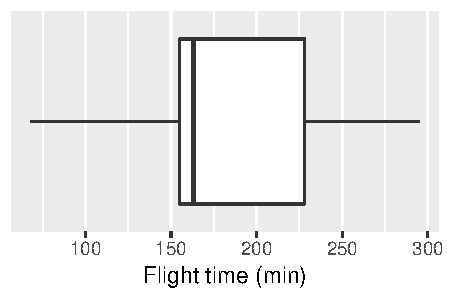
\includegraphics[width=\maxwidth]{figure/unnamed-chunk-20-1} 

\end{knitrout}

\end{frame}

% --------------------------------------------------- Slide --
\begin{frame}[fragile]{Quantile-quantile plots}

\begin{columns}[T,onlytextwidth]
    \column{0.45\textwidth}
    
\begin{itemize}
\item Quantile-quantile (Q-Q) plots compare two sets of quantiles
	\begin{itemize}
	\item Sample vs. sample
	\item Sample vs. theoretical quantiles
  \end{itemize}

\item Most common use is for comparison to normality
\end{itemize}

\column{0.45\textwidth}
\vspace{-1cm}
\hspace{1pc}
  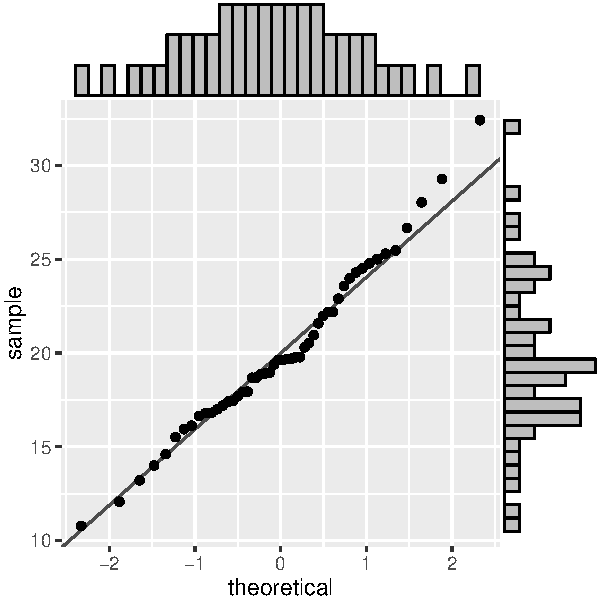
\includegraphics[width=1.05\linewidth]{figs/qqplot1.pdf}

\end{columns}
\end{frame}

% --------------------------------------------------- Slide --
\begin{frame}[fragile]{Interpreting Q-Q plots}

\begin{columns}[T,onlytextwidth]
    \column{0.45\textwidth}

\begin{itemize}
\item Deviations from the diagonal indicate differences between the distributions
\item[]
\item[]
\item[]
\end{itemize}

\vfill

\column{0.45\textwidth}
\vspace{-1cm}
\hspace{1pc}
\includegraphics[width=1.05\linewidth]<1>{figs/example-left-skew.pdf}
\includegraphics[width=1.05\linewidth]<2>{figs/example-right-skew.pdf}
\includegraphics[width=1.05\linewidth]<3>{figs/example-heavy-tail.pdf}
\end{columns}
\end{frame}


% --------------------------------------------------- Slide --
\begin{frame}[fragile]{Normal Q-Q plots}

\begin{knitrout}\small
\definecolor{shadecolor}{rgb}{0.969, 0.969, 0.969}\color{fgcolor}\begin{kframe}
\begin{alltt}
\hlkwd{ggplot}\hlstd{(}\hlkwc{data} \hlstd{= flights,} \hlkwc{mapping} \hlstd{=} \hlkwd{aes}\hlstd{(}\hlkwc{sample} \hlstd{= Delay))} \hlopt{+}
  \hlkwd{geom_point}\hlstd{(}\hlkwc{stat} \hlstd{=} \hlstr{"qq"}\hlstd{)}
\end{alltt}
\end{kframe}
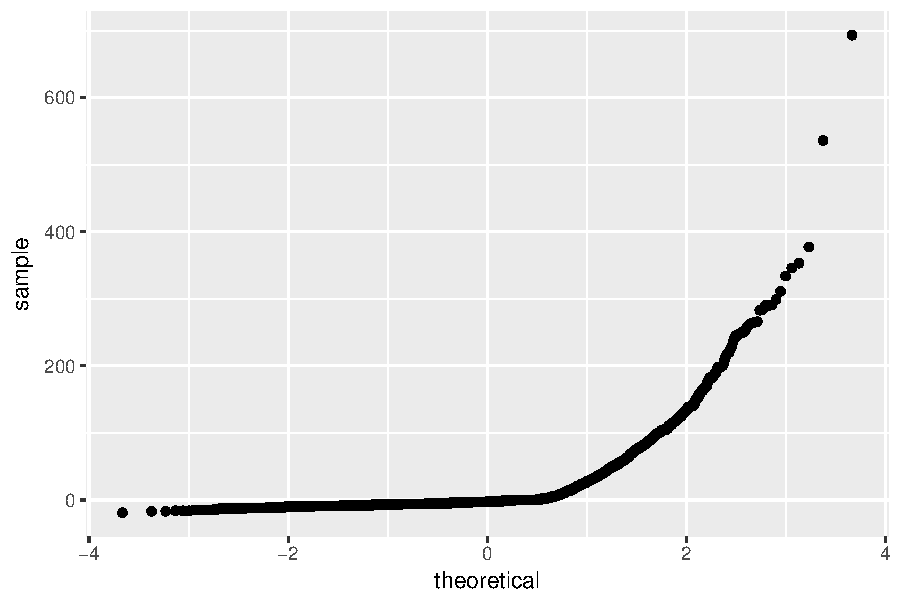
\includegraphics[width=3in,height=2in]{figure/unnamed-chunk-21-1} 

\end{knitrout}

\end{frame}

% --------------------------------------------------- Slide --
\begin{frame}[fragile]{Empirical CDFs}

For a sample consisting of $n$ observations $x_1, x_2, \ldots, x_n$, the ECDF is defined as

$$ \widehat{F} (x) = \dfrac{1}{n} \sum_{i=1}^n I_{(x_i \le x)} $$

\end{frame}

% --------------------------------------------------- Slide --
\begin{frame}[fragile]{Empirical CDFs}

\begin{knitrout}\small
\definecolor{shadecolor}{rgb}{0.969, 0.969, 0.969}\color{fgcolor}\begin{kframe}
\begin{alltt}
\hlkwd{ggplot}\hlstd{(}\hlkwc{data} \hlstd{= flights,} \hlkwc{mapping} \hlstd{=} \hlkwd{aes}\hlstd{(}\hlkwc{x} \hlstd{= Delay))} \hlopt{+}
  \hlkwd{stat_ecdf}\hlstd{(}\hlkwc{geom} \hlstd{=} \hlstr{"step"}\hlstd{)} \hlopt{+}
  \hlkwd{xlab}\hlstd{(}\hlstr{"Delay (min)"}\hlstd{)} \hlopt{+}
  \hlkwd{ylab}\hlstd{(}\hlstr{"F(x)"}\hlstd{)}
\end{alltt}
\end{kframe}
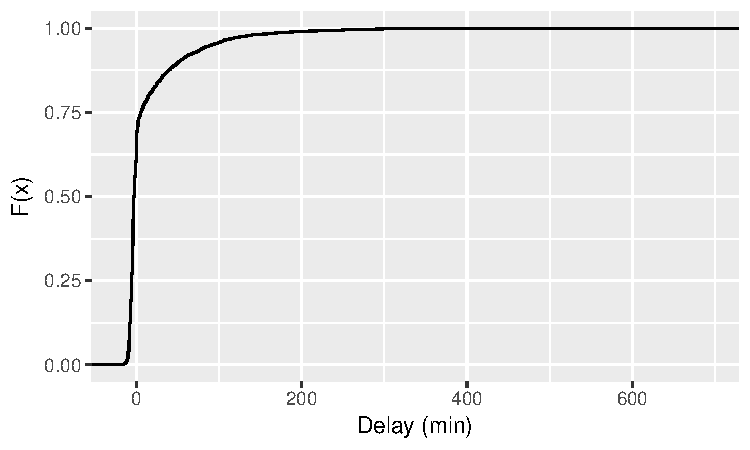
\includegraphics[width=3in,height=2in]{figure/unnamed-chunk-22-1} 

\end{knitrout}

\end{frame}

\end{document}
